\part{Práctica 1}
\section{Práctica 1-1}\label{p11}
\subsection{Actividad 1}\label{p11a1}
\begin{center}
    \parbox{12cm}{\justify\textit{
        Elija 3 bases de datos de la UCI Machine Learning Repository de las que hay en Moodle y transformelas a .arff, indicando en cada una de ellas qué procedimiento ha seguido.
    }}
\end{center}

\subsubsection{Consideraciones generales}\label{ssc:consideraciones-generales}
Para la realización de la tarea he tomado la decisión de editar manualmente los archivos utilizando Visual Studio Code y guardarlos con la extensión \code{.arff}. El paso a csv utilizando excel que se ha sugerido en clase supone varios cambios de formato en los que pueden aparecer diversos problemas como conflictos entre el separador de columnas CSV y el separador de decimales o miles, problemas con el carácter de salto de línea, codificación, etc.

Para conocer los identificadores y tipos de los atributos de cada base de datos he consultado el archivo \code{.names} del directorio de descarga de cada base de datos, que contiene el listado de campos con su nombre, su tipo y sus posibles valores, si procede. He consultado la especificación del formato \code{.arff} en la \href{https://www.cs.waikato.ac.nz/ml/weka/arff.html}{página correspondiente del manual de weka}. Como puede comprobarse en la figura \ref{fig:ejemplo-arff}, un archivo \code{.arff} consta de tres secciones:
\begin{figure}[H]
    \centering
    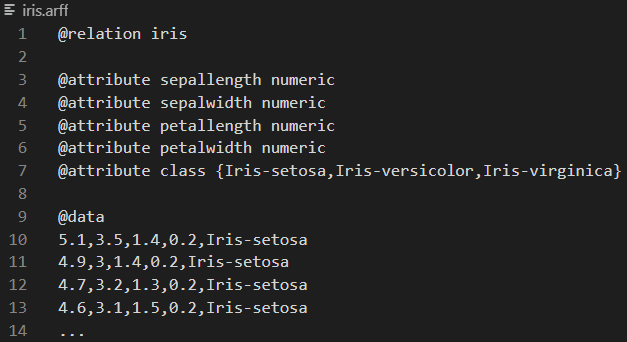
\includegraphics[scale=0.65]{ejemplo-archivo-arff}
    \caption{Ejemplo de archivo \code{.arff}}
    \label{fig:ejemplo-arff}
\end{figure}
\begin{enumerate}
    \item Identificación de la base de datos. Se trata de una línea con el token \code{@relation} seguido por un espacio y el nombre de la base de datos. Por ejemplo: \code{@relation breast-cancer}.
    \item Identificación de los atributos. Tantas líneas como atributos tenga la base de datos, cada una comienza con el token \code{@atribute} seguido del nombre del atributo y el tipo. Los tipos pueden ser:
        \begin{itemize}
            \item Numéricos: \code{@attribute <nombre\string_atributo>\space numeric}
            \item Cadenas de texto: \code{@attribute <nombre\string_atributo> \space string}
            \item Listas de etiquetas: \code{@attribute <nombre\string_atributo> \space\string{valor\string_1, valor\string_2, \dots\string}}
            \item Fechas: \code{@attribute <nombre\string_atributo>\space date [formato\string_de\string_fecha]}. El formato de fecha es opcional, y por defecto acepta ISO-8601 y ``yyyy-MM-dd'T'HH:mm:ss''.
        \end{itemize}
    \item Bloque de datos. Esta sección se inicia con una línea que contiene únicamente palabra clave \code{@data}. A continuación se encontrarán los registros dispuestos en líneas y con sus atributos separados por comas, en el mismo orden en que se han especificado en la cabecera:
    \begin{center}
        \parbox{5.1cm}{\code{@data \\
            v1a1, v1a2, \dots, v1aN \\
            v2a1, v2a2, \dots, v2aN \\
            \dots \\
            vMa1, vMa2, \dots, vMaN
        }}
    \end{center}

\end{enumerate}

\subsubsection{Base de datos \code{breast-cancer}}
Tras aplicar el tratamiento mencionado en el apartado \ref{ssc:consideraciones-generales} al archivo \code{breast-cancer.data} se ha obtenido el fichero \code{.arff} (fig. \ref{fig:breast-cancer-arff}) y una vez cargado en Weka (fig. \ref{fig:breast-cancer-weka}) y se han obtenido las siguientes conclusiones:

\begin{enumerate}
    \item La base de datos tiene 10 atributos, de los cuales el primero es la clase, que toma los valores ``no-recurrence-events'' y ``recurrence-events''. Convendría colocar la clase al final, que es su lugar por defecto.
    \item Los atributos son nominales basados en etiquetas (por ejemplo breast\_quad, menopause\dots) o en rangos numéricos (inv\_nodes, tumor\_size\dots). El atributo deg\_malig se podría poner como numérico ya que parece representar el grado de malignidad en un rango de 1 a 3, por lo que hay una distancia distinta entre los elementos (por ejemplo 1-2 y 1-3).
\end{enumerate}
\begin{figure}[ht]
    \centering
    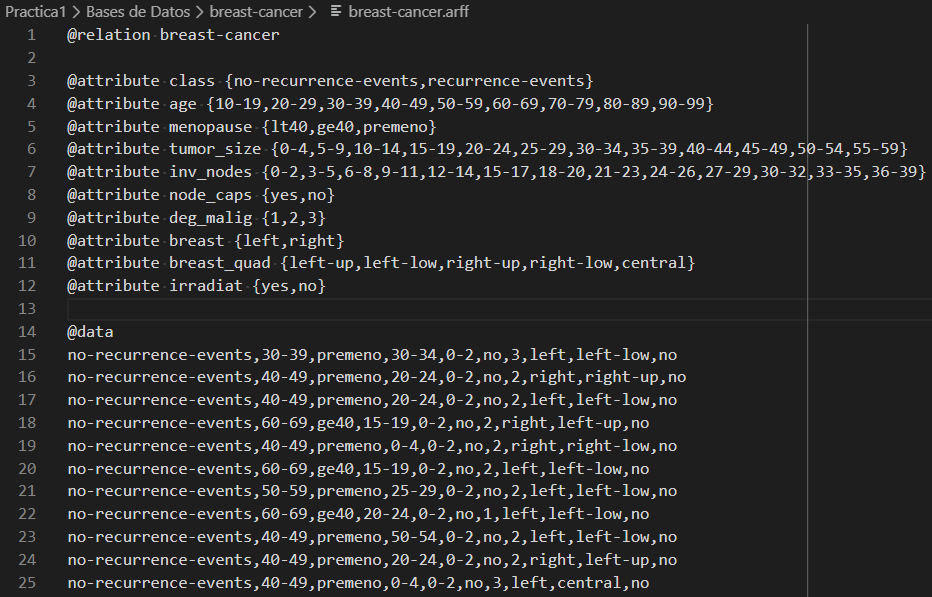
\includegraphics[scale=0.37]{breast-cancer-arff}
    \caption{Captura del archivo \code{breast-cancer.arff}.}
    \label{fig:breast-cancer-arff}
\end{figure}
\begin{figure}[ht]
    \centering
    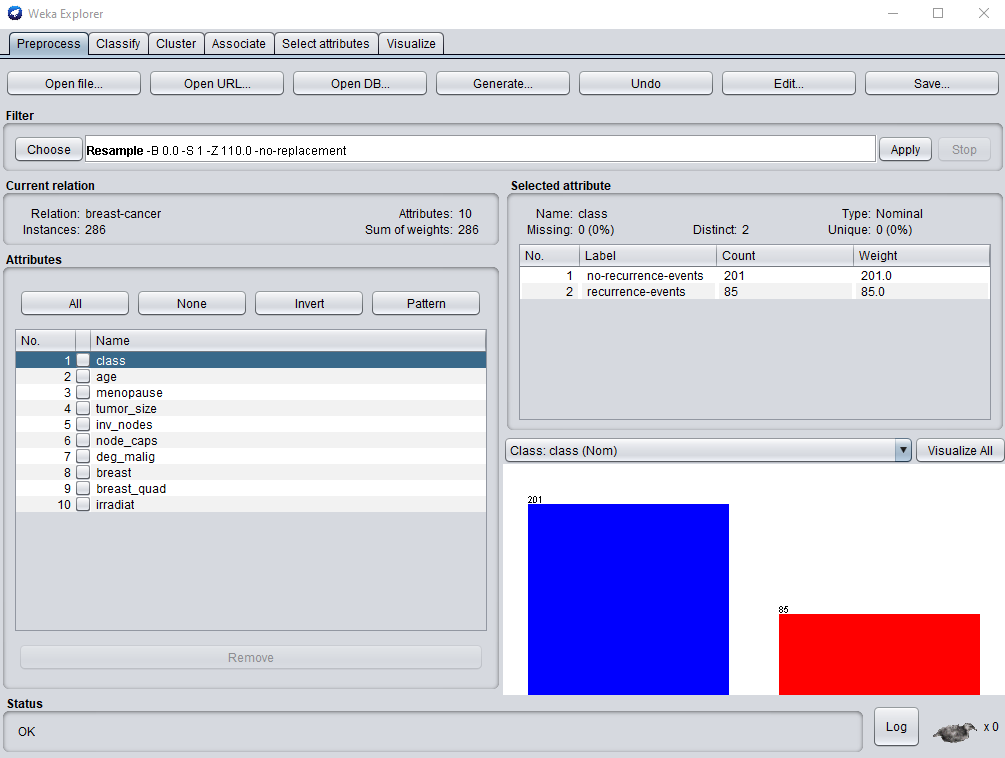
\includegraphics[scale=0.37]{breast-cancer-weka}
    \caption{Archivo \code{breast-cancer.arff} cargado en Weka.}
    \label{fig:breast-cancer-weka}
\end{figure}

\subsubsection{Base de datos \code{dermatology}}
Tras aplicar el tratamiento mencionado en el apartado \ref{ssc:consideraciones-generales} al archivo \code{dermatology.data} se ha obtenido el fichero \code{.arff} (fig. \ref{fig:dermatology-arff}) y una vez cargado en Weka (fig. \ref{fig:dermatology-weka}) y se han obtenido las siguientes conclusiones:

\begin{enumerate}
    \item La base de datos tiene 34 atributos independientes y una clase. En total hay 366 patrones.
    \item La mayoría los atributos son de tipo numérico con valores [0-3]. En la descripción se indica que los valores indican un grado obtenido de un análisis. El caso del atributo family-history es una excepción, ya que es nominal con valores 0 y 1 y representa si alguna de las enfermedades ha sido observada en la familia. Otra excepción es la edad, que siendo numérica, no está restringida al rango anterior.
    \item La clase toma valores de 1 a 6 y cada valor representa un diagnóstico diferente, por lo que es un dato nominal.
\end{enumerate}
\begin{figure}[ht]
    \centering
    \begin{minipage}{0.45\textwidth}
        \centering
        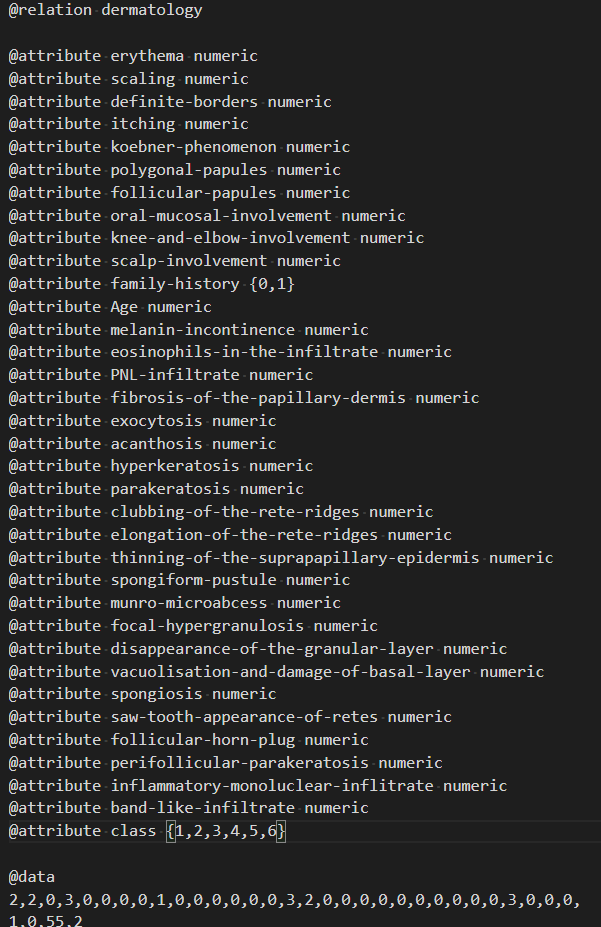
\includegraphics[scale=0.40]{dermatology-arff}
        \caption{Captura de \code{dermatology.arff}.}
        \label{fig:dermatology-arff}
    \end{minipage}\hfill
    \begin{minipage}{0.55\textwidth}
        \centering
        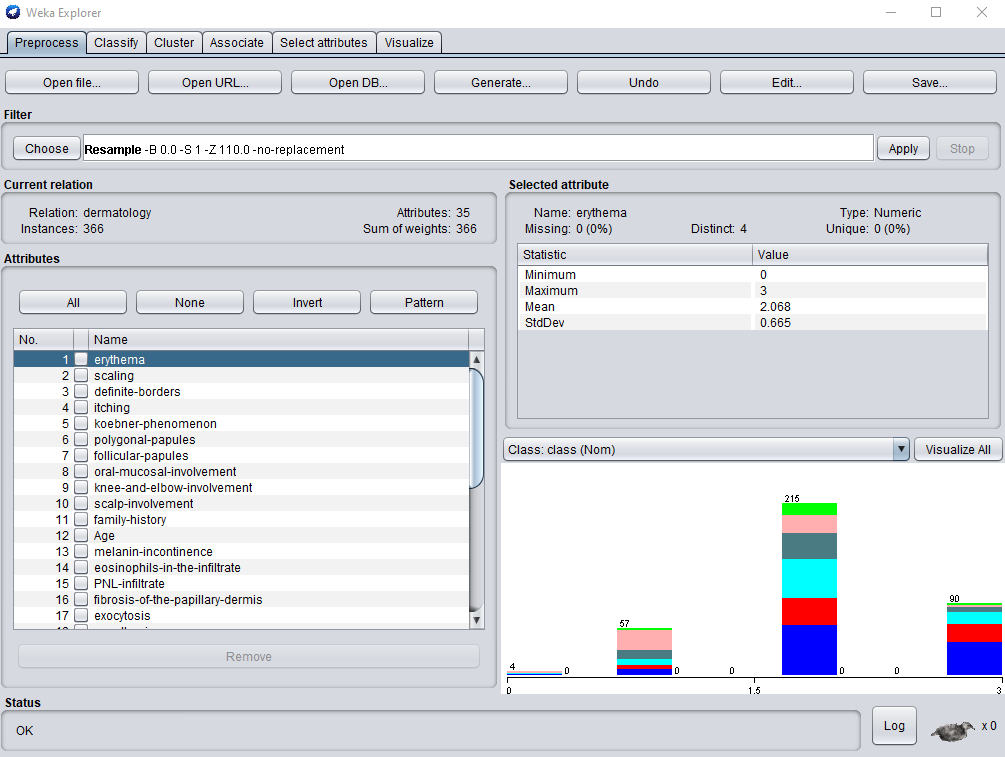
\includegraphics[scale=0.33]{dermatology-weka}
        \caption{Archivo \code{dermatology.arff} cargado en Weka.}
        \label{fig:dermatology-weka}
    \end{minipage}
\end{figure}


\subsubsection{Base de datos \code{wine}}
Tras aplicar el tratamiento mencionado en el apartado \ref{ssc:consideraciones-generales} al archivo \code{wine.data} se ha obtenido el fichero \code{.arff} (fig. \ref{fig:wine-arff}) y una vez cargado en Weka (fig. \ref{fig:wine-weka}) y se han obtenido las siguientes conclusiones:

\begin{enumerate}
\item La base de datos tiene 13 atributos independientes y una clase al principio.
\item Los atributos son numéricos continuos.
\item La clase toma valores 1, 2 o 3 con frecuencias 59, 71 y 48 respectivamente. Es un dato nominal
\end{enumerate}
\begin{figure}[h]
    \centering
    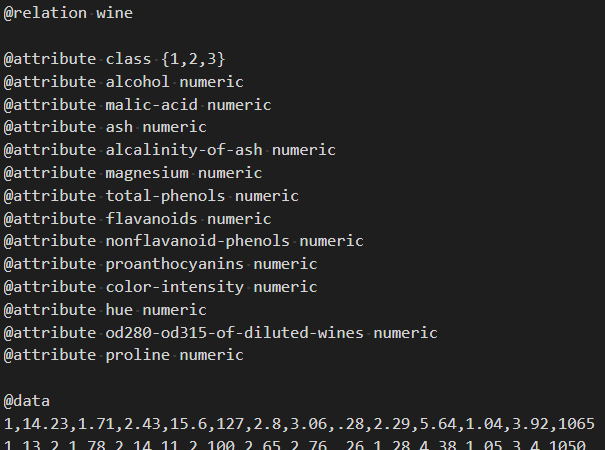
\includegraphics[scale=0.70]{wine-arff}
    \caption{Captura del archivo \code{wine.arff}.}
    \label{fig:wine-arff}
\end{figure}
\begin{figure}[h]
    \centering
    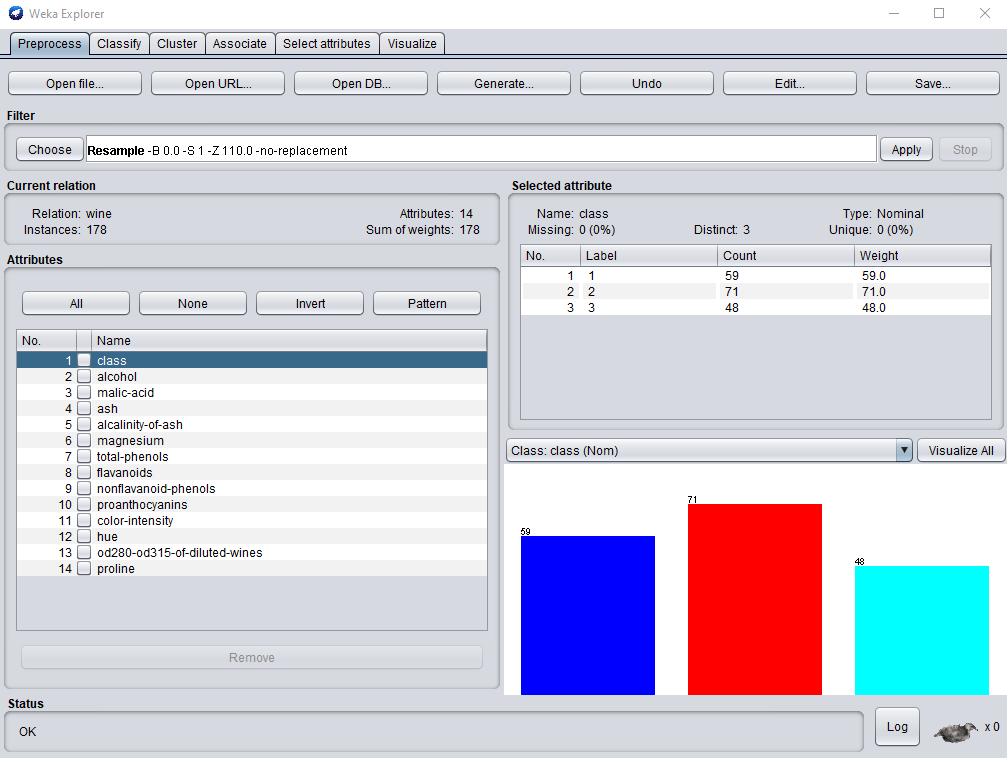
\includegraphics[scale=0.50]{wine-weka}
    \caption{Archivo \code{wine.arff} cargado en Weka.}
    \label{fig:wine-weka}
\end{figure}

\clearpage

\section{Práctica 1-2}\label{p12}
\subsection{Actividad 1}\label{p12a1}
\begin{center}
    \parbox{12cm}{\justify\textit{Elija 3 filtros No Supervisados de los que aparecen listados, expliquelos y describa cómo quedan los datos antes y después al aplicarlos sobre una o varias bases de datos.
    \begin{itemize}
        \item Consulte el UCI Machine Learning Repository para una descripción de la base de datos y la transformación a \code{.arff}
        \item Si no puede aplicar un filtro elegido en ninguna base de datos describa por qué, y constrúyase una base de datos ficticia y pequeña donde si pueda aplicarlo.
        \item Use capturas de pantalla, salidas de Weka y todo lo que considere necesario para sus ejercicios.
        \item La puntuación variará en función de la argumentación y dificultad de los filtros elegidos.
        \begin{enumerate}
            \item filters/unsupervised/attribute/Normalize
            \item filters/unsupervised/attribute/ReplaceMissingValues
            \item filters/unsupervised/attributes/NominalToBinary
            \item filters/unsupervised/intance/RemoveDuplicates
            \item filters/unsupervised/instance/Resample
            \item filters/unsupervised/attribute/Remove
            \item filters/unsupervised/attributes/RemoveUseless
        \end{enumerate}
    \end{itemize}
    }}
\end{center}

%-------------------------------------------------------------------------------
%-------------------------------------------------------------------------------
%-------------------------------------------------------------------------------

\subsection{Actividad 2}\label{p12a2}
\begin{center}
    \parbox{12cm}{\justify\textit{Elija 3 filtros Supervisados de los que aparecen listados, expliquelos y describa cómo quedan los datos antes y después al aplicarlos sobre una o varias bases de datos.
    \begin{itemize}
        \item Consulte el UCI Machine Learning Repository para una descripción de la base de datos y la transformación a \code{.arff}
        \item Si no puede aplicar un filtro elegido en ninguna base de datos describa por qué, y constrúyase una base de datos ficticia y pequeña donde si pueda aplicarlo.
        \item Use capturas de pantalla, salidas de Weka y todo lo que considere necesario para sus ejercicios.
        \item La puntuación variará en función de la argumentación y dificultad de los filtros elegidos.
        \begin{enumerate}
            \item filters/supervised/attribute/Discretize
            \item filters/supervised/attribute/NominalToBinary
            \item filters/supervised/instance/SpreadSubsample
            \item filters/supervised/instance/ClassBalancer
            \item filters/supervised/instance/Resample
        \end{enumerate}
    \end{itemize}
    }}
\end{center}